\chapter{Petites oscillations}

\section{Oscillations lin\'eaires libres}

\subsection{Amplitude et phase initiale}

En ayant $x(t=0) = x_{0}$ et $v(t=0) = v_{0}$ et en prenant la formule (\ref{EQ:21_8}), cela permet d'\'ecrire :
\be
	\begin{cases}
		x_{0} = a\cos\alpha \\
		v_{0} = -a\omega\sin\alpha
	\end{cases}
\ee
donc :
\be
	\begin{cases}
		\tan\alpha = \dfrac{-v_{0}}{\omega x_{0}} \\
		\\
		v_{0}^{2} + \omega^{2}x_{0}^{2} = a^{2}\omega^{2}\text{ donc } a =  \sqrt{x_{0}^{2} + \dfrac{v_{0}^{2}}{\omega^{2}}}
	\end{cases}
\ee

\subsection{Mol\'ecules diatomiques}

L'isotope d'un atome est ce m\^eme atome mais avec un nombre de neutrons diff\'erents. En cons\'equence, l'\'energie potentielle d'interactions n'est pas modifi\'ee. La formule (\ref{EQ:21_5}) appliqu\'ee aux deux composantes de la mol\'ecule diatomique devient :
\be
	\begin{cases}
		\ddot{x}_{1} + \frac{k}{m_{1}}x_{1}^{2} = 0 \\
		\ddot{x}_{2} + \frac{k}{m_{2}}x_{2}^{2} = 0 \\
	\end{cases}
\ee
En d\'efinissant $X = x_{1} + x_{2}$, nous avons :
\be
	\ddot{X} + k\left(\dfrac{1}{m_{1}} + \dfrac{1}{m_{2}}\right)X^{2} = 0
\ee
Et en appliquant le m\^eme raisonnement \`a la seconde mol\'ecule, nous avons :
\be
	\ddot{X'} + k\left(\dfrac{1}{m_{1}} + \dfrac{1}{m_{2}}\right){X'}^{2} = 0
\ee
ce qui permet finalement d'\'ecrire le rapport des fr\'equences entre les deux mol\'ecules diatomiques :
\be
	\dfrac{\omega'}{\omega} = \sqrt{\dfrac{k'}{k}\dfrac{m_{1}m_{2}(m'_{1} + m'_{2})}{m'_{1}m'_{2}(m_{1} + m_{2})}}
\ee
et comme il s'agit d'isotopes et que l'int\'eraction est donc la m\^eme alors $k = k'$.

\subsection{Fr\'equence d'oscillations pour un point sur une droite}

\begin{figure}[htb!]
	\begin{center}
		\begin{picture}(100,150)(0,0)
			%axis
			\linethickness{0.05mm}
			\multiput(0,0)(10,0){10}{\line(1,0){8}}\put(102,-2){$x$}
			\multiput(50,0)(0,10){10}{\line(0,1){8}}\put(55,47){$l$}
			%mass
			\put(40,100){\line(1,0){20}}\put(47,102){$A$}
			\put(25,0){\color{black}\circle*{10}}\put(20,-12){$m$}
			%spring
			\linethickness{0.05mm}
			\multiput(25,0)(3,12){8}{\line(1,4){2}}
			\multiput(27,10)(3,12){8}{\color{black}\circle*{1}}
		\end{picture}
		\caption{Oscillations contraintes par le d\'eplacement sur une droite}\label{FIG:21_EX3_1}
	\end{center}
\end{figure}

Quand le ressort est de longueur $l$, soit $x = 0$, alors il est tendu avec une force $F$. Puisque nous sommes dans l'hypoth\`ese de petites oscillations, soit de petits d\'eplacements de la masse $x$, alors la relation (\ref{EQ:5_8}) s'applique et permet d'\'ecrire : $U = F\delta l$ avec $\delta l$ l'allongement du ressort. En appliquant Pythagore :
\be
	(l + \delta l)^{2} = l^{2} + x^{2} \Leftrightarrow l^{2} + \delta l^{2} + 2l\delta l = l^{2} + x^{2} \Rightarrow \delta l = \dfrac{x^{2}}{2l}
\ee
en n\'egligeant $\delta l^{2}$ en premi\`ere approximation. L'\'energie totale de la masse $m$ vaut :
\be
	E = T + U = \dfrac{m}{2}\dot{x}^{2} + \dfrac{F}{2l}x^{2} = \dfrac{m}{2}\left(\dot{x}^{2} + \dfrac{F}{ml}x^{2}\right)
\ee
ce qui permet d'en conclure directement :
\be
	\omega^{2} = \dfrac{F}{ml}
\ee

\subsection{Fr\'equence d'oscillations pour un point sur un cercle}

\begin{figure}[htb!]
	\begin{center}
		\begin{picture}(100,150)(0,0)
			%lengths
			\linethickness{0.05mm}
			\put(50,90){\vector(0,-1){35}}
			\put(49,92){$l$}
			\put(50,102){\vector(0,1){48}}
			\put(50,23){\vector(0,-1){23}}
			\put(49,25){$r$}
			\put(50,33){\vector(0,1){22}}
			%circle
			\put(50,0){\line(-1,2){25}}
			\qbezier(50,55)(-5,50)(-5,0)
			\qbezier(50,55)(105,55)(105,0)
			%angle
			\qbezier(50,10)(47,10)(45,8)
			\put(43,15){$\varphi$}
			%mass
			\put(40,150){\line(1,0){20}}\put(47,152){$A$}
			\put(25,50){\color{black}\circle*{10}}\put(18,38){$m$}
			%spring
			\linethickness{0.05mm}
			\multiput(25,50)(3,12){8}{\line(1,4){2}}
			\multiput(27,60)(3,12){8}{\color{black}\circle*{1}}
		\end{picture}
		\caption{Oscillations contraintes par le d\'eplacement sur une portion de cercle}\label{FIG:21_EX3_2}
	\end{center}
\end{figure}

Nous utilisons les m\^emes hypoth\`eses et la m\^eme m\'ethode que pour l'exercice pr\'ec\'edent, \`a l'exception du fait que la situation g\'eom\'etrique oblige \`a utiliser la g\'en\'eralisation du th\'eor\`eme de Pythagore, \`a savoir la formule d'Al-Kashi :
\bea
	(l + \delta l)^{2} & = & (r + l)^{2} + r^{2} - 2(r + l)r\cos\varphi \nonumber \\
	l^{2} + \delta l^{2} + 2l\delta l & = & r^{2} + l^{2} + 2rl + r^{2} - 2(r + l)r\cos\varphi \Leftrightarrow 2l\delta l = 2r^{2} + 2lr - 2(r + l)r\cos\varphi \nonumber \\
	\delta l & = & \dfrac{r(r + l)(1 - \cos\varphi)}{l} = \dfrac{r(r + l)}{2l}\varphi^{2}
\eea
en utilisant l'hypoth\`ese de petits d\'eplacements qui permet de n\'egliger la quantité $\delta l^{2}$ et d'utiliser le d\'eveloppement en s\'erie de Taylor au premier ordre pour $(1 - \cos\varphi)$ tel que :
\be
	\cos\varphi = \cos(0) - \sin(0)\varphi - \dfrac{1}{2}\cos(0)\varphi^{2} \Leftrightarrow \cos\varphi = 1 - \dfrac{1}{2}\varphi^{2}
\ee
L'\'energie totale s'\'ecrit :
\bea
	E & = & T + U = \dfrac{mr{2}\dot{\varphi}^{2}}{2} + \dfrac{r(r + l)F}{2l}\varphi^{2} \nonumber \\
	& = & \dfrac{m}{2}\left(r^{2}\dot{\varphi}^{2} + \dfrac{r(r + l)F}{ml}\varphi^{2}\right) = \dfrac{m}{2}\left((r\dot{\varphi})^{2} + \dfrac{(r + l)F}{mlr}(r\varphi)^{2}\right)
\eea
donc, la fr\'equence d'oscillations s'\'ecrit :
\be
	\omega^{2} = \dfrac{(r + l)F}{mlr}
\ee

\subsection{Oscillations du pendule plan}

Pour d\'eterminer la fr\'equence des oscillations, nous reprendrons la formule (\ref{EQ:13_EX3_1}) pr\'ealablement \'etablie dans ce contexte, voir la figure (\ref{FIG:1_2}). L'\'energie totale s\'ecrit alors dans sa forme g\'en\'erale :
\be
	E = \dfrac{m_{2}l^{2}\dot{\varphi}^{2}}{2}\left(1 - \dfrac{m_{2}\cos^{2}\varphi}{(m_{1} + m_{2})}\right) - m_{2}gl\cos\varphi
\ee
qui peut se d\'evelopper en utilisant l'approximation au second ordre $\cos\varphi = 1 - \dfrac{1}{2}\varphi^{2}$ :
\be
	E = \dfrac{m_{2}l^{2}\dot{\varphi}^{2}}{2}\left(1 - \dfrac{m_{2}}{(m_{1} + m_{2})}(1 + \frac{1}{4}\varphi^{4} - \varphi^{2})\right) - m_{2}gl(1 - \dfrac{1}{2}\varphi^{2})
\ee
ou en n\'egligeant les ordres sup\'erieurs \`a 2 :
\bea
	E & = & \dfrac{m_{2}l^{2}\dot{\varphi}^{2}}{2}\left(\dfrac{m_{1} + m_{2} - m_{2}}{(m_{1} + m_{2})}\right) - m_{2}gl + \dfrac{1}{2}m_{2}gl\varphi^{2} \nonumber \\
	& = & \dfrac{m_{1}m_{2}l^{2}}{2(m_{1} + m_{2})}\dot{\varphi}^{2} + \dfrac{1}{2}m_{2}gl\varphi^{2} - m_{2}gl = \dfrac{m_{2}}{2}\left(\dfrac{m_{1}l^{2}}{m_{1} + m_{2}}\dot{\varphi}^{2} + gl\varphi^{2}\right) - m_{2}gl
\eea
Relation qui permet d'en d\'eduire la fr\'equence :
\be
	\omega^{2} = \dfrac{gl(m_{1} + m_{2})}{m_{1}l^{2}} = \dfrac{(m_{1} + m_{2})g}{m_{1}l}
\ee

\subsection{Trajectoire dans un champ de pesanteur telle que la fr\'equence d'oscillation ne d\'epend pas de l'amplitude}

Soit $m$ la masse de la particule en mouvement dans un champ de pesanteur et $s$ la coordon\'ee curviligne le long de la trajectoire. Dans ce cas, l'\'energie cin\'etique $T$ vaut $\frac{1}{2}m\dot{s}^{2}$, l'\'energie potentielle $U$, $\frac{1}{2}ks^{2}$ et la fr\'equence des oscillations $\omega^{2} = \frac{k}{m}$. Dans un champ de pesanteur o\`u $y$ est la coordonn\'ee verticale, l'\'energie potentielle vaut $mgy$, aussi, nous pouvons d\'ej\`a poser :
\be
	mgy = \dfrac{k}{2}s^{2} \Leftrightarrow s = \sqrt{\dfrac{2mg}{k}y} \Leftrightarrow \dfrac{\mathrm{d}s}{\mathrm{d}y} = \sqrt{\dfrac{mg}{2ky}} = \sqrt{\dfrac{g}{2\omega^{2} y}}
\ee
Par d\'efinition, $\mathrm{d}s^{2} = \mathrm{d}x^{2} + \mathrm{d}y^{2}$, soit :
\be
	\mathrm{d}x^{2} = \left(\left(\dfrac{\mathrm{d}s}{\mathrm{d}y}\right)^{2} - 1\right)\mathrm{d}y^{2} \Rightarrow x = \int{\sqrt{\left(\dfrac{\mathrm{d}s}{\mathrm{d}y}\right)^{2} - 1}\mathrm{d}y} = \int{\sqrt{\dfrac{g}{2\omega^{2} y} - 1}\mathrm{d}y}
\ee
En posant :
\be
	\begin{cases}
		y = \dfrac{g}{4\omega^{2}}(1 - \cos\xi) \\
		\mathrm{d}y = \dfrac{g}{4\omega^{2}}\sin\xi\mathrm{d}\xi
	\end{cases}
\ee
$x$ se formule alors :
\be
	x = \int{\sqrt{\dfrac{2}{(1 - \cos\xi)} - 1}\dfrac{g}{4\omega^{2}}\sin\xi\mathrm{d}y} = \dfrac{g}{4\omega^{2}}\int{\sqrt{\dfrac{1 + \cos\xi}{(1 - \cos\xi)}}\sin\xi\mathrm{d}y}
\ee
De plus, sachant que pour un angle $\alpha$, $\sin\alpha = \sqrt{1 - \cos^{2}\alpha} = \sqrt{(1 + \cos\alpha)(1 - \cos\alpha)}$, alors :
\be
	x = \dfrac{g}{4\omega^{2}}\int{(1 + \cos\xi)\mathrm{d}y} = \dfrac{g}{4\omega^{2}}(\xi + \sin\xi)
\ee

\begin{figure}[htb!]
	\begin{center}
		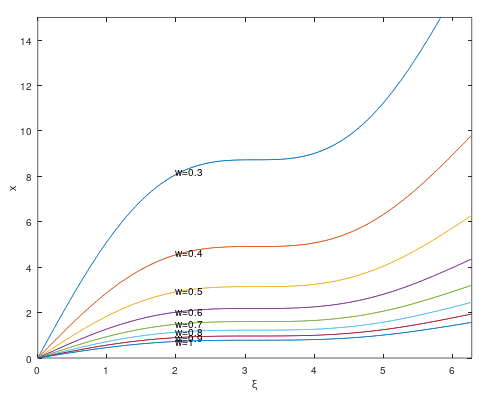
\includegraphics[width=10cm]{chapter_05_paragraph_21_exercice_6}
		\caption{Exemples de trajectoire pour diff\'erentes valeurs de fr\'equence telle que cette derni\`ere ne d\'epende pas de l'amplitude)}\label{FIG:5_21_EX6}
	\end{center}
\end{figure}

\section{Oscillations for\'ees}

Dans les excercices suivants, le syt\`eme se trouve \`a l'\'equilibre et au repos \`a l'instant $t = 0$, i.e. $x(t = 0) = 0$ et $\dot{x}(t = 0) = 0$.

\subsection{Mouvement dans le cas d'une force ext\'erieure non born\'ee dans le temps}

Il s'agit de d\'eterminer les oscillations forc\'ees, $x(t)$, d'un syst\`eme dues \`a une force $F(t)$ dans diff\'erents cas pr\'ecis.

\subsubsection{$F = F_{0}$}

Dans ce cas, l'\'equation (\ref{EQ:22_2}) s'\'ecrit :
\be
	\ddot{x} + \omega^{2}x = \dfrac{F_{0}}{m}
\ee
dont la solution g\'en\'erale sans second membre peut s'\'ecrire : $a\cos(\omega t + \alpha)$ et une int\'egrale particulière constante, dont la d\'eriv\'ee seconde par rapport au temps est \'evidemment nulle, telle que $\omega^{2}x = \frac{F_{0}}{m} \Leftrightarrow x = \frac{F_{0}}{m\omega^{2}}$. Les conditions initiales permettent de d\'eduire :
\be
	\begin{cases}
		\dot(x)(0) = 0 \Leftrightarrow -\frac{F_{0}}{m\omega^{2}}\omega\sin\alpha = 0 \Leftrightarrow \sin\alpha = 0 \Leftrightarrow \alpha = 0 \\
		x(0) = 0 \Leftrightarrow a + \frac{F_{0}}{m\omega^{2}} = 0
	\end{cases}
\ee
ce qui donne comme solution :
\be
	x = \frac{F_{0}}{m\omega^{2}}(1 - \cos(\omega t))
\ee

\subsubsection{$F = at$}

La solution de l'\'equation (\ref{EQ:22_2}) est consiste en :
\begin{itemize}
	\item la solution g\'en\'erale sans second membre : $x_{0} = a\cos(\omega t + \alpha)$
	\item l'int\'egrale particuli\`ere : $x_{1} = bt$ qui permet d'arriver \`a : $0 + \omega^{2}bt = \frac{F_{0}}{m}t \Leftrightarrow b = \frac{F_{0}}{m\omega^{2}}$
\end{itemize}
Les condtions initialies permettent les d\'eductions suivantes :
\be
	\begin{cases}
		x(0) = 0 \Leftrightarrow \Leftrightarrow a\cos\alpha = 0 \Leftrightarrow \alpha = \pm\frac{\pi}{2} \\
		\dot{x}(0) = 0 \Leftrightarrow -a\omega\sin\alpha + \frac{F_{0}}{m\omega^{2}} = 0 \Leftrightarrow a = \pm\frac{F_{0}}{m\omega^{3}}
	\end{cases}
\ee
donc :
\be
	x(t) = \dfrac{F_{0}}{m\omega^{3}}(\omega t + \cos(\omega t \pm \pi/2)) \Leftrightarrow x(t) = \dfrac{F_{0}}{m\omega^{3}}(\omega t \pm \sin(\omega t))
\ee

\subsubsection{$F = F_{0}e^{-\alpha t}$}

\subsubsection{$F = F_{0}e^{-\alpha t}\cos\beta t$}

\subsection{Mouvement dans le cas d'une force ext\'erieure born\'ee dans le temps}

\section{Oscillations des syst\`emes \`a plusieurs degr\'es de libert\'e}

\subsection{Oscillations d'un syst\`eme \`a deux degr\'es de libert\'e}

\subsection{Petites oscillations d'un pendule double oscillant dans un plan}

\subsection{Trajectoire dans un champ central $\propto r^{2}$}\label{PAR:23_EX3}